\section{RESULTADOS E DISCUSSÕES}

\lipsum[1-1]

\subsection{Exemplos de gráficos e figuras}

Para inserir figuras no \LaTeX é utilizado o comando \textsc{includegraphics}. Para indexar essa figura precisamos do ambiente \textsc{figure}. Veja como exemplo a Figura \ref{fig:figura1}. Neste template, as figuras devem ser armazenadas fisicamente no diretório \textsc{graphics}.
Ajuste a label e a legenda adequadamente.

\begin{figure}   %\captionsetup{singlelinecheck=false,justification=justified,format= hang,font=normalsize}
    \caption{Exemplo de figura.}
    \vspace{-0.5 cm}
    \begin{center}
    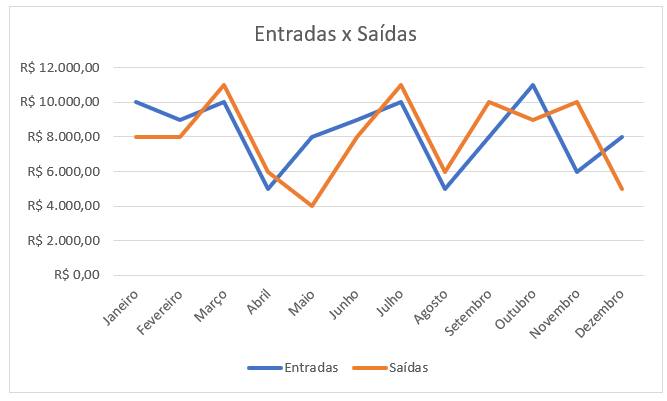
\includegraphics[scale=0.8]{graphics/exemploFigura1.png}
    \end{center}
    \vspace{-0.3 cm}
    \small{Fonte: EXCELEASY (2024).}
    \label{fig:figura1}
\end{figure}

\subsection{Exemplo de tabelas}

Pra Quadros ou Tabelas, recomenda-se  a ajuda do site ``Tables Generator'' (TABLES GENERATOR, 2024). Além disso, para indexação é necessário o ambiente \texttt{table}. Veja um exemplo na Tabela

\begin{table}[h]
\centering
\caption{Exemplo de tabela.}
\begin{tabular}{|l|l|l|l|}
\hline
& \textbf{A} & \textbf{B} & \textbf{C} \\
\hline
1 & 11         & 12         & 13         \\
2 & 0          & 2          & 3          \\
3 & 25         & 26         & 27    \\     
\hline    
\end{tabular}
\vspace{0.2 cm}

\small{Fonte: A autora.}
\end{table}

\normalsize



\subsection{Exemplo de Programas, Scripts ou Algoritmos}

Programas ou Scripts podem ser escritos em \LaTeX usando o pacote \texttt{lstlisting}. É importante que esse pacote seja configurado adequadamente de acordo com a linguagem de programação utilizada. Como exemplo, veja o Programa que está escrito em Python. Neste template, a configuração do pacote está discponível no arquivo \texttt{estrutura.tex}.

\begin{lstlisting}[caption={Função Eliminação de Gauss},label={prog:gauss},language=Python]
import numpy as np

def gauss(n, A, b):#algoritmo do livro do Ruggiero
    '''
    supor que o elemento que estah na posicao akk 
    eh diferente de zero no inicio da etapa k
    '''
    A_copy = A.copy()
    b_copy = b.copy()
    for k in range(0,n-1):
        for i in range(k+1,n):
            m = float(A_copy[i][k]/A_copy[k][k])
            for j in range(k,n):
                A_copy[i][j] = float(A_copy[i][j]-
                    float(m*A_copy[k][j]))
            b_copy[i] = float(b_copy[i]) - float(m*b_copy[k])
            A_copy[i][k] = 0
    #fase da resolucao
    return retroativa(n,A_copy,b_copy)
\end{lstlisting}
\small{Fonte: A autora}

\normalsize


 \lipsum[1-2]



